\section{Astoria}
\begin{frame}{Measuring AS-level adversaries against Tor}
	\begin{itemize}
		\item Multiple Autonomous Systems (AS) collude with each other
	performing time based attacks and collecting asymmetric data.

		\item Up to 40\% of circuits constructed by the current Tor
	client are vulnerable to AS-level attackers.

		\item Connections  from  China  were  found  to  be  most  vulnerable 
	to AS-level attackers with up to 86\% of
	all  Tor  circuits.
	\end{itemize}
\end{frame}


\begin{frame}{Mitigating AS-level adversaries against Tor}{ASes
correlations}

	Connections between ASes are negotiated as business arrangements.
\begin{figure}
			\centering
			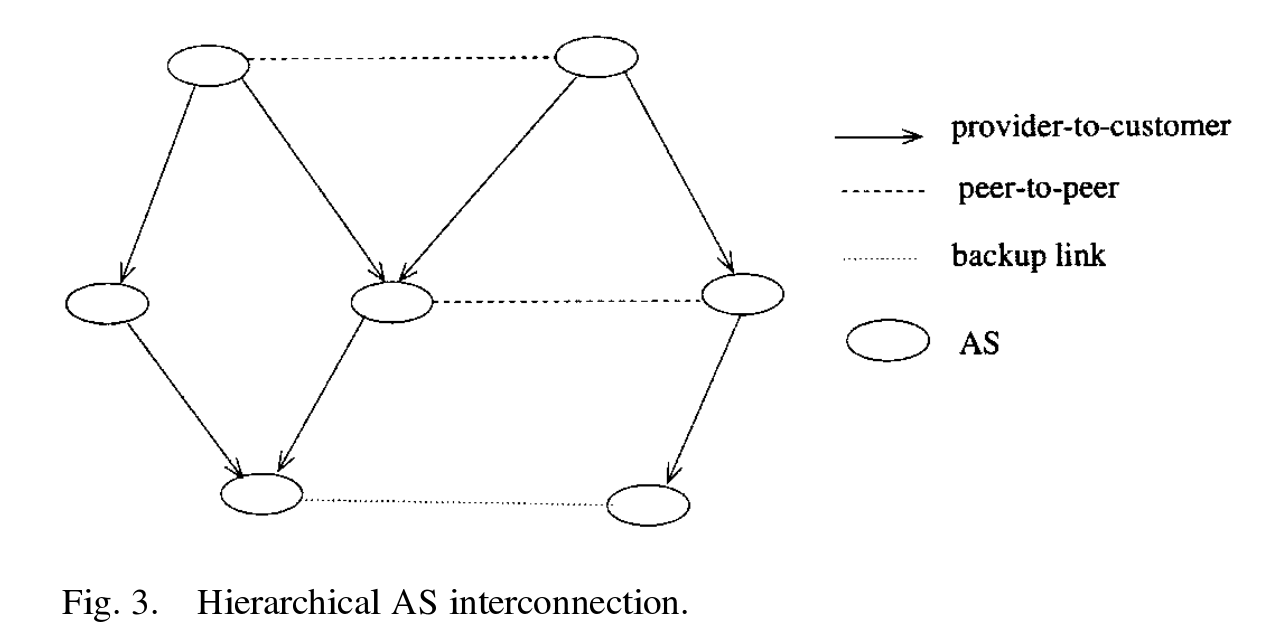
\includegraphics[scale=0.18]{imgs/as_graph.png}
		\end{figure}

	\begin{block}{The idea}
		Building a graph of ASes correlations to identify vulnerable
	paths.
	
	\end{block}
	\end{frame}

\begin{frame}{Astoria}

	\begin{itemize}
		\item Use of path prediction to avoid Tor vulnerable paths.\\
	i.e. The entry node and the exit node may be selected together if their ASes 
	are unrelated to each others.
		\item Able to perform  load-balancing at least as well as the vanilla Tor
client.
	\end{itemize}


\end{frame}


%\section{Other ORs and technologies}
%\subsection{HORNET}
	%change OR model
	%faster because does not encrypt the payload for each relay (only
	%the headers)
	%protects also against timing attacks?

\section{Open Problems}
\begin{frame}{Open Problems}
	User awareness on privacy and anonimity.
		\begin{figure}
				\centering
				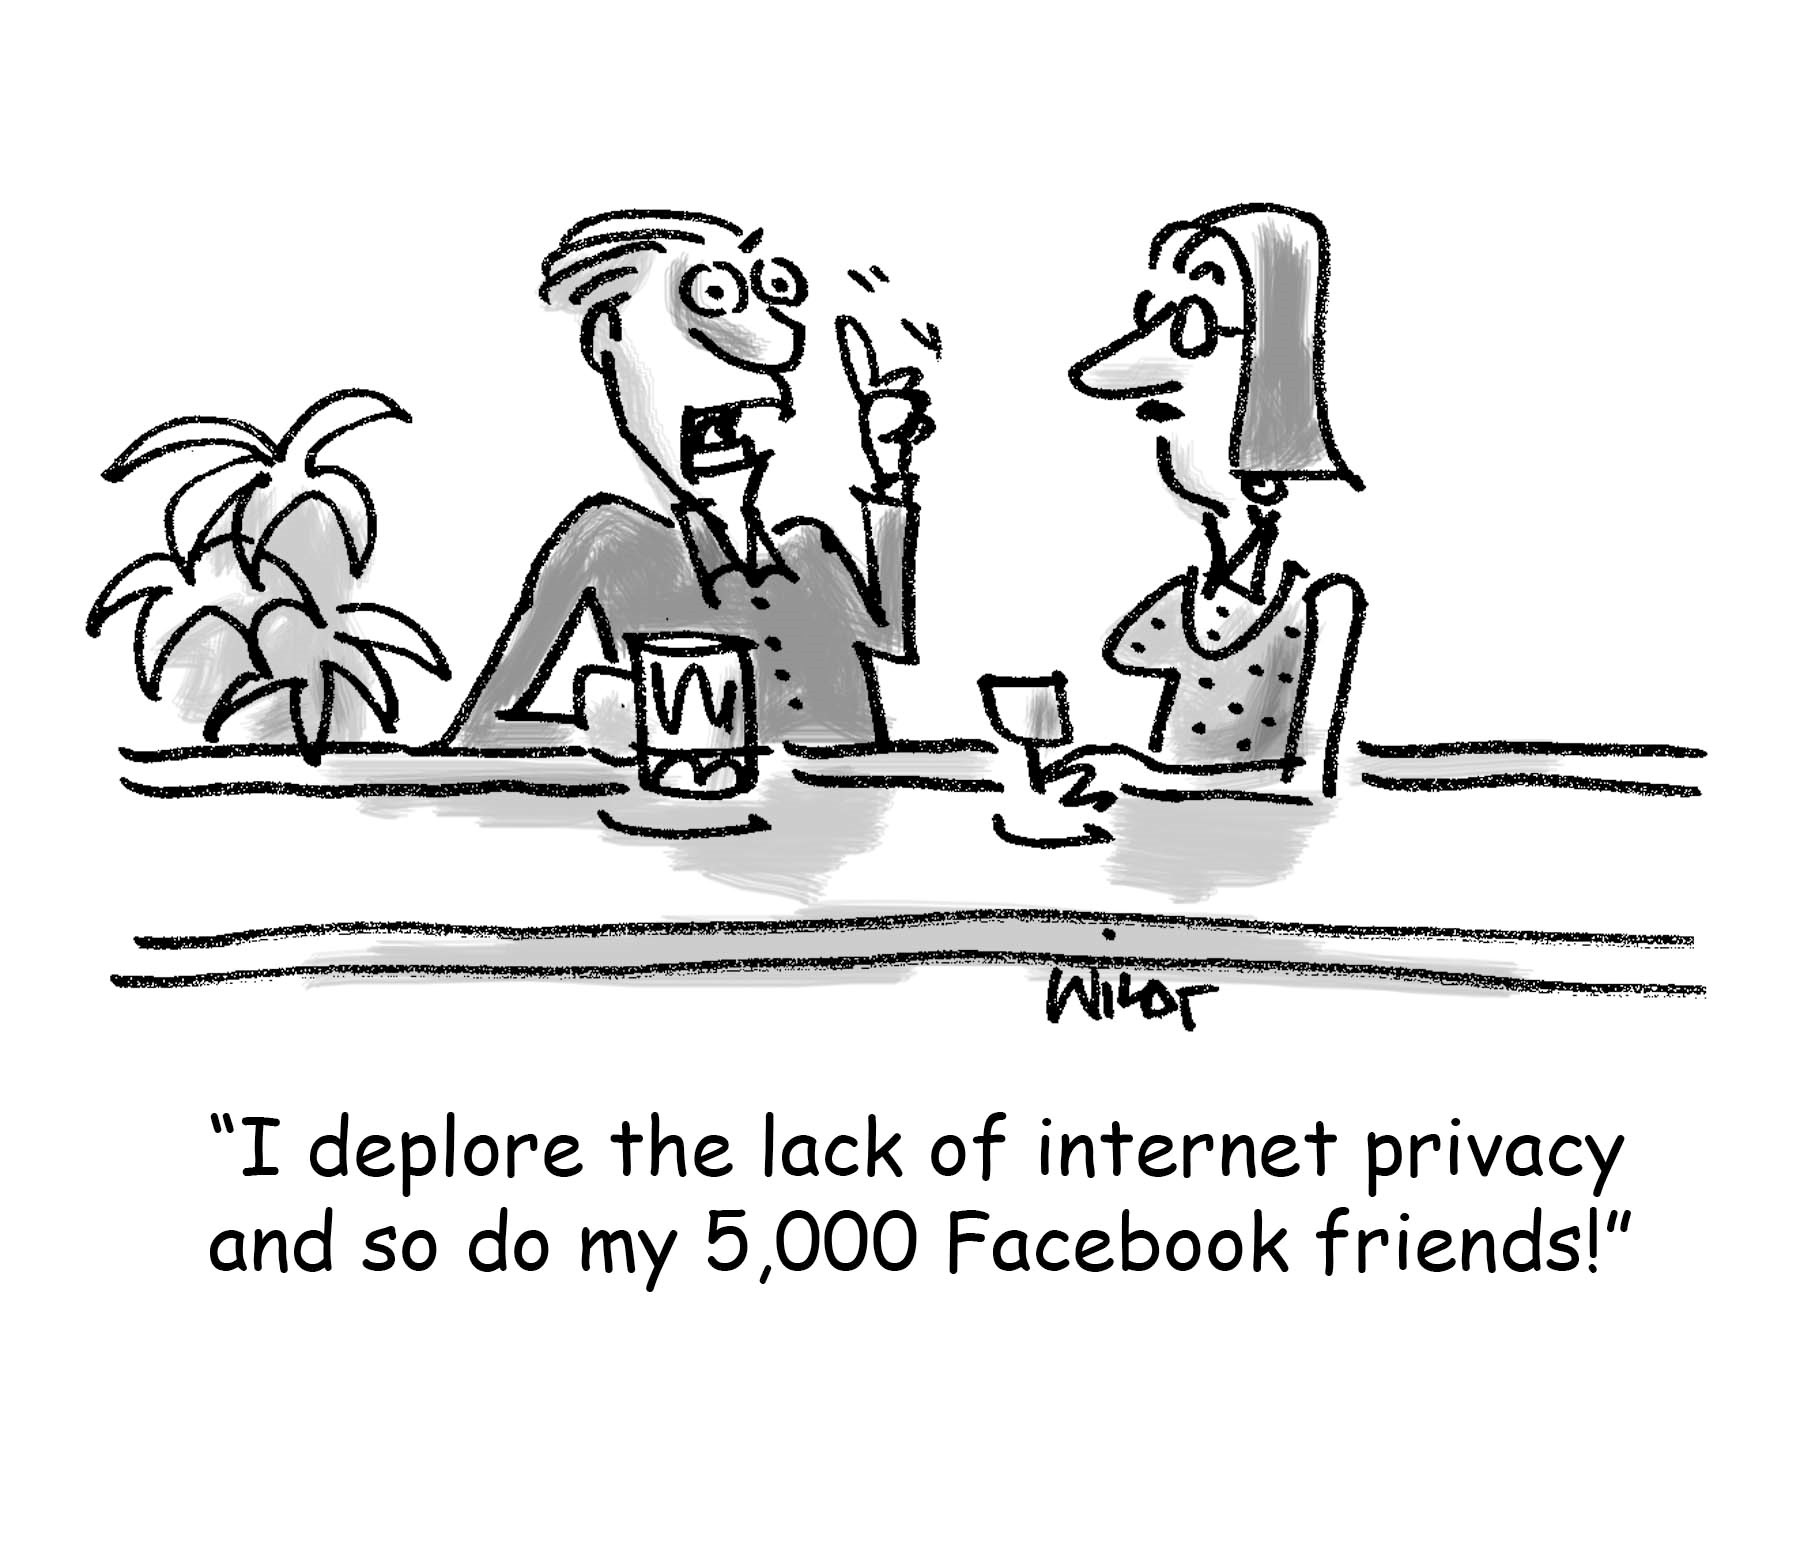
\includegraphics[scale=0.50]{imgs/comic1.jpg}
			\end{figure}
	
\end{frame}

\begin{frame}{Open Problems}
	
	\begin{figure}
		\centering
		
\includegraphics[scale=0.50]{imgs/comic2.jpg}
	\end{figure}

	Need of \emph{real} privacy laws and investments on network
security solutions. (IPSec, anti surveillance architectures, etc.)
\end{frame}
